\documentclass[12pt]{article}

\usepackage{graphicx}
\usepackage{minted}

\graphicspath{ {./Imagenes/} }

\author{Pablo Vargas Bermudez}

\begin{document}

\pagestyle{empty}

\section*{Redacción del problema}

Realiza un programa que muestre un tablero de ajedrez ( 8 X 8
celdas). Recuerda que la celda blanca de la esquina superior izquierda
deberá ser blanca.

\section*{Código}

\subsection*{Clase Gui}

\inputminted{Java}{Gui.java}

\subsection*{Clase de prueba}

\inputminted{Java}{Prueba.java}

\section*{Ejecución}

\subsection*{Tablero 8x8}

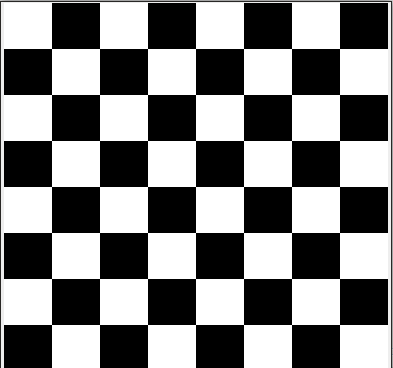
\includegraphics[width=\textwidth]{Corrida1.png}

\subsection*{Tablero 4x4}

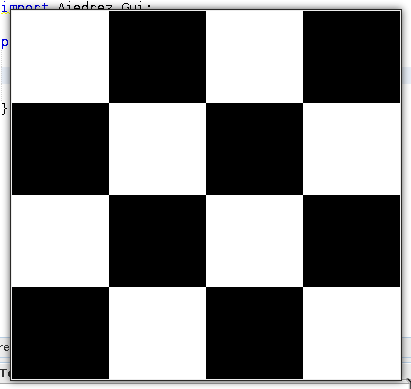
\includegraphics[width=\textwidth]{Corrida2.png}

\subsection*{Tablero 2x4}

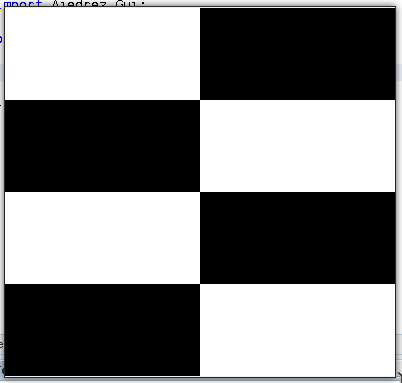
\includegraphics[width=\textwidth]{Corrida3.png}

\end{document}
